\documentclass[twocolumn]{ltjsarticle}
\usepackage{dcolumn}
\usepackage[dvipdfmx]{graphicx}
\usepackage[dvipdfmx]{color}

\begin{document}
\title{\bf\vspace{-3cm}
{トレーディングカードゲームにおける
\\初期手札枚数差による勝率変化調査} 
}
\author{\vspace{-1cm}髙橋昇太\footnotemark[1] 
阿原一志\footnotemark[1]}
\date{}
\twocolumn[
\maketitle
\small{\textbf{概要:}トレーディングカードゲーム(TCG)には,手札枚数や個々のカードの攻撃力など,様々なパラメータが存在する.
これらの値は一般に勝敗に大きく関わるとされているが,科学的実証は報告されていない.
そこで本研究では,パラメータ変更による勝率の変化について調査する手法の提案を行う.%後で変更
本論文では特に,初期手札の枚数差を意図的に生じさせ,どのように勝率が変化するかを調査した.
その結果,初期手札枚数が多いプレイヤーは勝率が高くなる傾向があることが明らかになった.
  \\\vspace{0.1cm}
  \noindent
  \textbf{キーワード:}不完全情報ゲーム,トレーディングカードゲーム(TCG), ゲーム人工知能
}
\begin{center}
  \vspace{0.3cm}
\large \textbf{A Study on the Effect of the Number of Cards in the Starting Hand
  \\on the Winning Percentage in Trading Card Games
  }
\author{\textrm{
  \vspace{0.1cm}\\Shota Takahashi\footnotemark[1]  Kazushi Ahara\footnotemark[1]}
  \vspace{0.1cm}
}
\end{center}
\small{\\\textbf{Abstract:}In trading card games (TCG), there are various parameters, such as the number of cards
in players' hands and the attack power of each card. Although we generally consider these values to
play essential roles in winning or losing, little quantitative evidence has been researched. In this
study, we propose a method to investigate the change of winning rate by changing parameters. This
paper examines how the winning rate changes by intentionally changing the number of starting cards
in their hands. As a result, we find that the player with more starting cards has significantly higher
winning percentages.
\\
\noindent
\textbf{Keywords:}Imperfect Information Game, Trading Card Game(TCG),Game Artificial Intelligence
\vspace{0.2cm}
}]
\section{はじめに}
\small{
  トレーディングカードゲーム(以下,TCG)とは
「Magic: the Gathering」などを例とする 2 人用不完全
情報ゲームで,近年では「Hearthstone」や「Shadowverse」
のようにオンライン上で遊べるものもあり,その裾
野が広がっている.TCG は囲碁や将棋のようにター
ン制で進むが,使用するカードを各プレイヤーが選
べ(使用するカードの束をデッキと呼ぶ),デッキから
ランダムに引くカードの種類,いわゆる「引き」によ
り戦局や戦略が左右されるという点が TCG の大
きな特徴である.
\\TCG には様々なパラメータが存在する.手札の枚
数やターン数,出したカードの攻撃力値やプレイヤ
ーの体力,デッキの枚数などがそれにあたる.これら
のパラメータの値は対戦結果に大きな影響を及ぼす
とされている.実際に TCG 運営会社は,試合中のパ
ラメータを調整するようなルールやカード能力を設
定している.例えば「Hearthstone」では,先手後手の
有利差を少なくするためにコインというパラメータ
調整カードを後手プレイヤーに初期配布するという
ルールになっている.同様の理由で「Shadowverse」
では,先手プレイヤーは手札を 4 枚,後手プレイヤー
は手札を 5 枚から試合開始となる.またこれらのゲ
ームでは,特定のカードやデッキの使用率,勝率が著
しく高かった場合,ナーフと呼ばれるカード能力の下方修正が行われるケースもある.このように,パラ
メータの値は試合結果に大きな影響を及ぼすことが
わかっている.一方これらの事象(調整ルールやナー
フ)は経験から来る考えであり,定量的な検証は公開
されていない.
\\そこで本研究では,パラメータの変更による勝率
変化を実験により測定し,実際にどれくらいハンデ
ィキャップが生じるかを統計的に調査する.この手
法を用いることにより,パラメータが試合に与える影響をより具体的な数値で観察できる.
これは,カード能力調整をはじめとした運営開発に貢献できるほか,
TCG 初心者へ向けた良質なハンデ調整などに応用できるようになると筆者は考
える.本論文では,種種のパラメータの中から特に初
期手札の枚数差による勝率変化について詳細に記す.
}
\section{関連研究}
\small{
  \verb#[1]#では,カード間の相性測定の提案並びにその有効
性について実験を行った.相性の数値化による比較
は,パラメータの比較と関連があり,今後の実験にお
いて検証する要因になりうる.\verb#[2]#では Magic: The Gathering において,お互いにデ
ッキの構成がわかっている場合,モンテカルロ木探
索(MCTS)と Determinization を用いることが有効な
手法であることを明らかにした.本実験でも,この手
法を参考にプレイヤーエージェントの作成を行った.
}
\section{システム説明}
\small{
  本研究の実験は, Hearthstone のシミュレーション
エンジンである fireplace を基に,筆者らが独自に改
良を加えた fireplaceAharalab [3]を用いた.このシミュ
レーションエンジンは,2019 年の Hearthstone 通常プ
レイのルールに沿って実装したもので,ハンター,ド
ルイド,メイジ,ニュートラルカードの 95\%以上のカ
ード効果を再現した.これにより,Hearthstone のルー
ルを基にした汎用的なプレイの実験が可能である.
}
\section{評価実験}
\small{
  本実験では,同じアルゴリズムを持つ 2 つのプレイ
ヤーエージェント A と B を用意し対戦を行う.A の
初期手札は 4 枚,B の初期手札は 4+α枚とする.こ
こでαを枚数差と呼ぶことにし,αは 1≦α≦5 の整
数であるとする.αの範囲は,ゲームのルール上手札
の枚数の上限が 10 枚であることを考慮し最初のター
ンに上限を超えない範囲を指定した.対戦数は 1 セ
ット 30 戦として,これを各枚数差ごとに 10 セット
行う.本実験で使用したプレイヤーエージェントは A
と B ともに Vector エージェントである.これは,自
身の体力や相手の場にいるカードの攻撃力などいく
つかのデータを取り出し,これらの重みづけ和によ
って,一手読みを実行し,その結果最も良い点数の行
動を行うエージェントである.
本実験ではプレイ環境の違いを顕在化させるため,
使用したデッキは A と B ともに同じデッキである.
また,試合開始時に行われる手札交換(マリガン)は行
わず,先攻後攻はランダムに決定される.ハースストーン特有のコインは使用しない事とした。同条件下において差が生じるかを検証するためである。
実験の結果に対し平均勝率と分散を計算し,実際に初期手札枚
数差による勝率変化を見る.
}
\section{結果と考察}
\small{
  実験結果を以下に示す.
}
\begin{table}[h]
  \centering
  \caption{初期手札枚数差によるBの1セットあたりの平均勝利数と分散}
  \begin{tabular}{clll}
    α &平均勝利数(勝)& 分散\\
    \hline \hline
    \centering
    1&\multicolumn{1}{c}{16.50}&\multicolumn{1}{l}{15.17}\\
    2&\multicolumn{1}{c}{16.70}&\multicolumn{1}{l}{6.01}\\
    3&\multicolumn{1}{c}{20.10}&\multicolumn{1}{l}{3.88}\\
    4&\multicolumn{1}{c}{22.30}&\multicolumn{1}{l}{12.23}\\
    5&\multicolumn{1}{c}{22.30}&\multicolumn{1}{l}{2.21}\\
    \hline%小数点でそろえたいいいいい怒
  \end{tabular}
\end{table}
%図を入れます

\begin{figure}[h]
  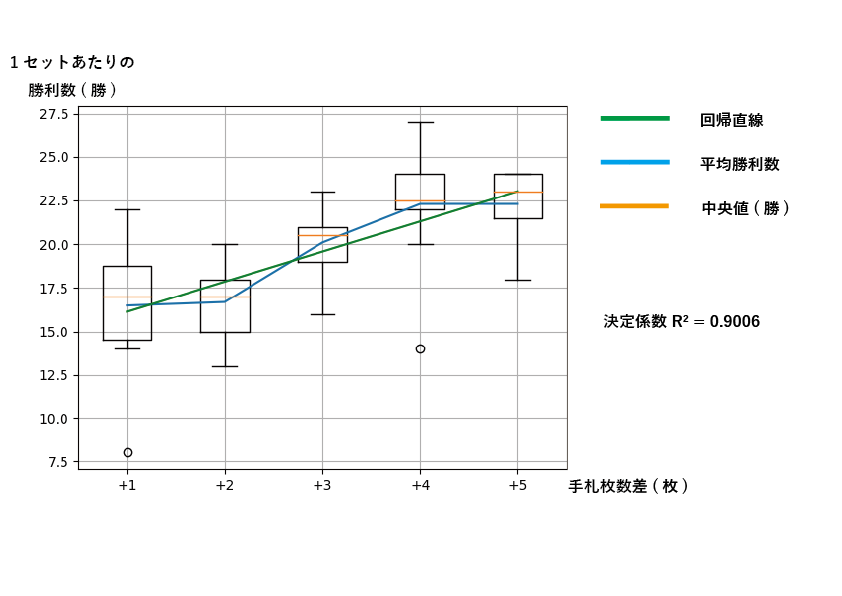
\includegraphics[width=30mm]{graph1.png}
  \caption{AとBの手札枚数差とBの平均勝利数}
  \end{figure}
\small{\leavevmode\\
表1は,αの値による平均勝率と分散をまとめたものである.
αが大きくなるにつれて分散が小さくなり,高い勝率を維持できることが分かった.
また,図1はAとBの手札の枚数差とBの勝利数を箱ひげ図で表し,回帰直線と平均勝利数,決定係数を表示したものである.
手札枚数差と勝率の相関係数は0.943と非常に高く,手札枚数差が大きくなるほどBが勝つ傾向が見られた.
次にこの結果に至った経緯を考察する.手札が多いことのメリットとしてプレイ行動の選択肢の多さが挙げられる.
今回の分散と相関係数の結果から,手札が多くなるほど安定して勝利数が増えることが観察された.
これは,選択肢が多いと状況に応じた柔軟なプレイができ,より安定した戦略で対戦を進めることができると考えられる.
特に,αが4から5にかけて分散がより小さくなっていた.
このことから,一定の初期枚数差があるとより顕著に勝利しやすくなることが考えられる.
また,回帰直線の傾きが 0.57 であることから,初期枚数 1 枚の増加につき 0.5 勝分の平均勝率の上昇が見込める.
このことから,初期枚数の違いによる有利さを定量化することができたと考えられる.
}

\section{議論と結論}
\small{
  本論文は,初期手札枚数差と勝率の関係について実
験及び考察を行った.その結果,同様なプレイヤーで
あれば,初期手札枚数が多い程ゲームに安定して勝
つことが分かった.また,この結果から TCG のパラ
メータ変更において,ハンディキャップの定量化が
できたといえる.つまり,他のパラメータの差も,同
様の実験で検証することができると筆者は考える.
一方で議論すべき問題点もある.
第一に,片方のプレイヤーにしか手札を増やして
実験していない点である.実際の TCG では,一部例
外はあるものの,カードのルールによってお互いに
手札を増やしながら対戦することが想定される.今
後,手札枚数による調査を行うときは,両プレイヤー
の手札を増やしつつ手札枚数差がある際の勝率を観
測することも検討すべきである.また,本実験では手
札枚数差を生じさせたのは対戦開始前であった.手
札枚数差を生じさせるタイミングを変更した場合の
実験も検討が必要である.
第二に,特定のデッキ,プレイヤーエージェントを
固定して実験を行った点である.プレイヤーごとに
異なるデッキ,エージェントを用いても同様の結論
は見込めるものの,初期手札 1 枚当たりの勝率への
寄与のばらつきはさらに実験によって確かめなけれ
ばならない.これらの実験も検討すべきである.
}
\section{
  参考文献
}
\small{
  \verb#[1]#山田豊大,阿原一志(2020)”トレーディングカー
  ドゲームにおけるバニラカードを用いたカード間の相性計測”,ゲームプログラミングワークショップ2020論文集
  \\
  \verb#[2]#Peter I. Cowling [ほか].(2012).“Ensemble
  Determinization in Monte Carlo Tree Search for the
  Imperfect Information Card Game Magic: The Gathering”.
  IEEE Transactions on Computational Intelligence and AI
  in Games (241-257),4(4)
  \\
  \verb#[3]#fireplaceAharalab(GithubURL:https://github.com
  /aharalabMeiji/fireplaceAharaLab)
  \\
  \verb#[4]#Vectorエージェント(GithubURL:https://
  github.com/aharalabMeiji/fireplaceAharaLab/wiki)
  

  
}

\footnotetext[1]{総合数理学部先端メディアサイエンス学科}
\end{document}